%\textsf{Web of Things architecture \cite{Wot2017arch}, Thing Description \cite{Wot2017td} and
%scripting API \cite{Wot2017script}.}
The WoT architecture\cite{Wot2017arch} defines three basic entities
that can be organized into various configurations and topologies 
based on a concrete deployment scenario:

\begin{itemize}
	\item A \textbf{WoT Thing} represents a physical or virtual IoT device 
        and exposes a network-facing API for interaction.
	Each WoT Thing has an associated Thing Description (TD)\cite{Wot2017td}. 
        A TD encodes a set of metadata describing relevant information about a Thing,
        such as semantic categorization, available interactions, and communication and security mechanisms.
	A typical example of a WoT Thing might be a garage door controller.
        Such a controller would provide a number of actions that can be performed on a garage door, 
        i.e. \textit{open}, \textit{close}, etc. and would provide network interfaces to invoke
        each of these.
        Typically a WoT Thing plays the network role of a server as it responds to
        but does not initiate interactions.
	\item A \textbf{WoT Client} is an entity that wants to perform an action on a WoT Thing.
	It is able to consume a TD provided by (or for) a WoT Thing and issue actions on 
        the target's network interfaces.
	For example a WoT Client might be a browser or an application on a user's smartphone
        that allows the user to invoke one of the actions provided by the garage door controller. 
	\item A \textbf{WoT Servient} can be viewed as a combination of a client and server:
        an entity that is both providing one or more WoT Thing interfaces (as a server) and
        at the same time is able to operate as WoT Client to invoke interactions on other WoT Things.
	An example of a WoT Servient would (a service running on a) home gateway device 
        that acts as a WoT Client towards home appliance WoT Things
        (such as different lights and sensors) and also exposes some higher level
        virtual devices (such as the collection of all the lights in the living room)
        in form of additional WoT Things available for a WoT Client running on a user's smartphone.
\end{itemize}

Internally a typical architecture of a WoT Servient is shown in Figure~\ref{fig-fservient}. 
In addition to a Thing Description (TD) it also has WoT Binding Templates 
that can be used to instantiate a TD for a particular IoT protocol binding, 
such as OCF, HTTP(S), COAP etc. 
Internally a WoT Servient can also host a WoT Runtime and
a WoT Scripting API.
The WoT Scripting API is an optional component that allows 
implementing logic of an application Servient in a standardized way
using a higher-level programming language (such as JavaScript). 

\begin{figure}[!t]
\centering
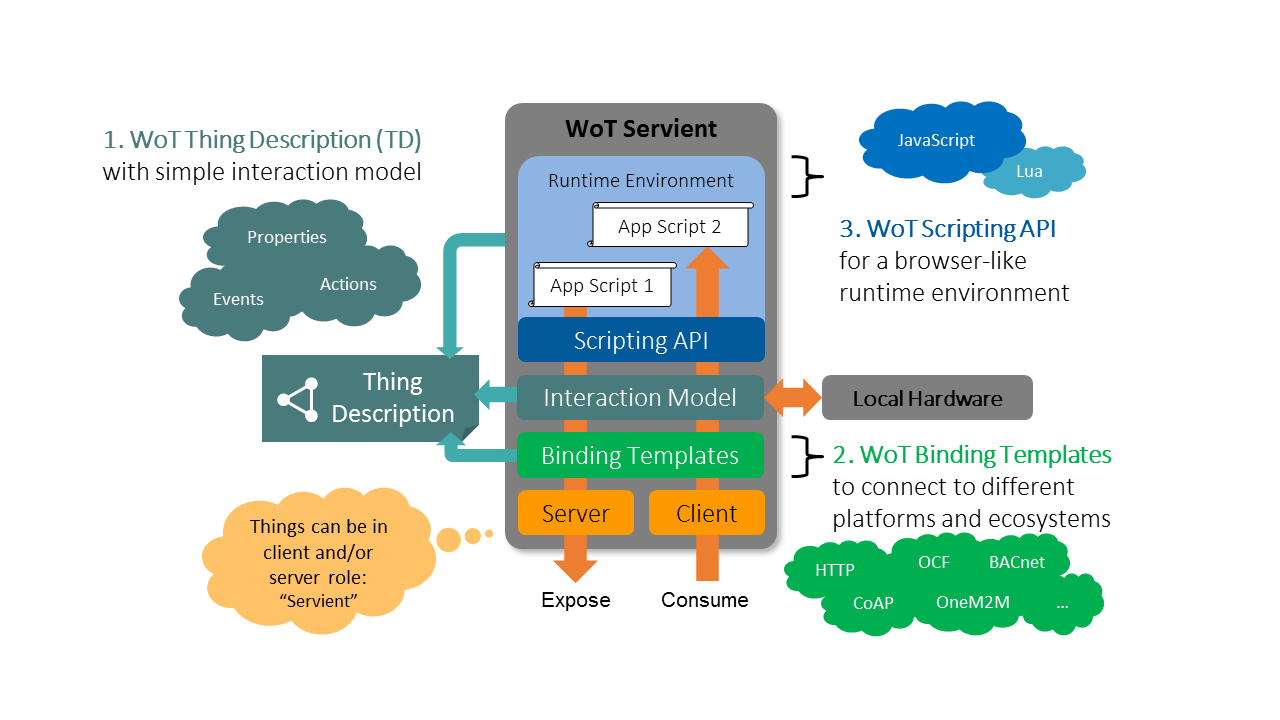
\includegraphics[width=4in]{figures/wot-servient.png}
\caption{WoT Servient architecture}
\label{fig-fservient}
\end{figure}


